\subsection{Funktionale Verschlüsselung}\label{sec:funktionale_verschlüsselung}

Eine weitere Methodik, Berechnungen auf verschlüsselten Daten durchzuführen, ist die sogenannte funktionale Verschlüsselung.
Diese wurde 2011 von Boneh \etal \cite{P-44} vorgestellt.
Funktionale Verschlüsselung erlaubt es, eine im Voraus definierte, mathematische Funktion $f$ eines Klartextes zu berechnen, wobei nicht der Klartext als Input der Funktion genutzt wird, sondern der Geheimtext. 
Anders als bei der homomorphen Verschlüsselung, liegt das Ergebnis der Berechnung nicht verschlüsselt vor, sondern als Klartext.
Funktionale Verschlüsselung basiert auf folgenden vier Schritten \cite{P-44}:
\begin{compactenum}
    \item \textbf{Setup: } In einem Vorbereitungsschritt wird ein Public Key $pk$ und ein Master Secret Key $msk$ erzeugt.
    \begin{equation*}
        (pk, msk) \xleftarrow{} Setup
    \end{equation*}
    \item \textbf{Schlüsselgenerierung: } Der Master Secret Key kann nun genutzt werden, um einen spezifischen Secret Key $sk$ für eine definierte Funktion $f$ zu erzeugen.
    \begin{equation*}
        sk \xleftarrow{} Keygen(msk, f)
    \end{equation*}
    \item \textbf{Verschlüsselung: } Der Public Key $pk$ wird genutzt, um den Klartext $x$, auf welchem die Berechnung durchgeführt werden soll, zu verschlüsseln.
    \begin{equation*}
        c \xleftarrow{} Enc(pk,x)
    \end{equation*}
    \item \textbf{Entschlüsselung: } Die Entschlüsselung des Geheimtextes $c$ mittels des spezifischen Secret Key $sk$ entspricht hierbei der Berechnung der Funktion $f$ mit dem Parameter $x$.
    \begin{equation*}
        f(x) \xleftarrow{} Dec(sk,c)
    \end{equation*}
\end{compactenum}

Die Berechnung der Funktion erfolgt demnach während der Entschlüsselung.
Das System, welches die Entschlüsselung vornimmt, sieht dementsprechend nur die verschlüsselten Daten sowie das Ergebnis der Berechnung, nicht jedoch den unverschlüsselten Eingabewert.

Die ersten Ansätze, funktionale Verschlüsselung und neuronalen Netze zu verbinden, fokussierten sich auf die Inferenz der Modelle, welche in Kapitel \ref{sec:krypto_inferenz} genauer betrachtet werden.
Ein Framework für das Training des Modells mit dem Namen CryptoNN wurde jedoch von Xu \etal \cite{P-53} vorgestellt.
Dieses ermöglicht, ein Modell auf einem fremden Server, \zB in einer Public Cloud, zu trainieren, ohne dass der Provider des Servers Einblick in die Daten erhält.
Dabei wird eine funktionale Verschlüsselung genutzt, welche die Berechnung des Skalarprodukts und zusätzlich auch die Grundrechenarten (Addition, Subtraktion, Multiplikation und Division) von zwei Vektoren elementweise ermöglicht.
Kombiniert ermöglicht dies, alle notwendigen Berechnungen beim Training des Modells durchzuführen.
CryptoNN führt dabei 3 Rollen ein: Autorität, Client und Server. 
Dabei ist es auch möglich, dass es mehrere Clients gibt, die zusammen ein Modell trainieren.
Gibt es jedoch nur einen Client, so übernimmt dieser auch die Rolle der Autorität.
Die Autorität ist dafür zuständig, einen Master Secret Key $msk$ und einen Public Key $pk$ zu erzeugen, den Public Key $pk$ an den Client zu verteilen und bei Bedarf spezifische Secret Keys $sk_n$ zu erzeugen und an den Server weiterzugeben.
Der Client ist Besitzer der Daten und verschlüsselt diese vor der Übergabe an den Server mit dem Public Key $pk$. 
Der Server führt das tatsächliche Training des Modells durch.
Beim Forward-Pass wird funktionale Verschlüsselung zur Berechnung der Neuronen der ersten Hidden Layer genutzt.
Dafür fordert der Server einen spezifischen Secret Key $sk_n$ an, der die Berechnung der ersten Schicht ermöglicht.
Der restliche Forward-Pass erfolgt unverschlüsselt.
Wenn der Client auch das Label verschlüsselt, kann die Berechnung der Verlustfunktion für jedes Output Neuron ebenfalls verschlüsselt erfolgen.
% Abbildung \ref{fig:cryptonn} zeigt das CryptoNN Framework.
% \begin{figure}[!htb]
%     \centering
%     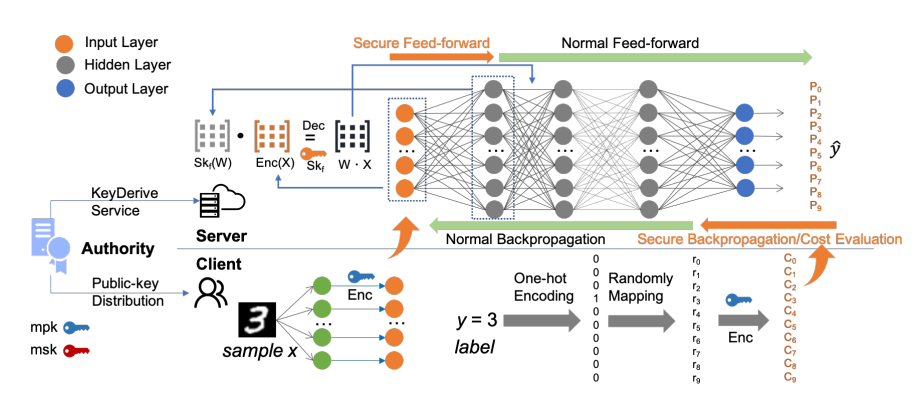
\includegraphics[width=\textwidth]{figures/cryptoNN}
%     \caption{CryptoNN Framework \cite{P-53}}
%     \label{fig:cryptonn}
% \end{figure} 

Ein Problem des CryptoNN Frameworks ist jedoch, dass davon ausgegangen wird, dass der Server kein Angreifer ist, der effektiv versucht Daten zu extrahieren.
Ansonsten könnte dies dazu führen, dass der Server diverse White-Box Angriffe (Kapitel \ref{sec:angriffe}) durchführen könnte, da das Modell unverschlüsselt vorliegt.
Die Methodik ist demnach darauf ausgelegt, dafür zu sorgen, dass Clients Daten verschlüsselt übertragen können und diese nicht beispielsweise von dem Cloud-Provider mitgelesen werden können.


